\section{What  \mixin Generates}\label{sec:translation}

We now show what the \mixin annotation generates. We present a formal definition for
most of the generated methods; however in our formalism we do not consider
% setters, so we do not formally define the generation of the setters.
%We do not include
casts or \Q@instanceof@, so we do not include the \Q@with@ method.
For the same reason we do not include \Q@void@ returning setters, since they are just a minor variation over the more interesting fluent setters, and they would require special handling just for the conventional \Q@void@ type.

\hl{Furthermore, we introduce \textbf{@ObjWeak}, which is only an annotation for illustrating the translation, hence is not implemented in Lombok. By this, the real translation is divided into two parts: \textbf{@Obj} automatically refines the return types only, and \textbf{@ObjWeak} generates the constructor method $\QM{of}$. In the source code, the only annotation \textbf{@Obj} combines both of the work and finishes the translation at a time.}

\subsection{Translation Function}

Two translation functions for the two parts are presented as follows:

\noindent$\begin{array}{l}
\InTextDef{18em}{[\![\mixinAnn\ \QM{interface}\ \C_0\ \QM{extends}\ \Cs\ \oC \methods\ \cC ]\!]
}{
\weakAnn\ \QM{interface}\ \C_0\ \QM{extends}\ \Cs\ \oC
\methods\ \methods' \cC
}\\
\InTextWith{\methods'=\otherMethod(\C_0,\methods)}
\end{array}$

\noindent\hl{To translate an interface annotated by \mixin, we add some other methods for type refinement, then add a new annotation \textbf{@ObjWeak} to the interface.}

\noindent$\begin{array}{l}
\InTextDef{18em}{[\![\weakAnn\ \QM{interface}\ \C_0\ \QM{extends}\ \Cs\ \oC \methods\ \cC ]\!]
}{
\emptyset\ \QM{interface}\ \C_0\ \QM{extends}\ \Cs\ \oC
\methods\ \method' \cC
}\\
\InTextWith{\valid(\C_0),\QM{of}\notin\dom(\methods) \mbox{ and } \method'=\ofMethod(\C_0)}
\end{array}$

\noindent\hl{To translate an interface annotated by \textbf{@ObjWeak}, we add the $\QM{of}$ method.}
However, first of all we check if the interface is valid for annotation:

\noindent$\valid(\C_0)$  holds if $\forall \m\in\dom(\C_0),$ if $\mh\QM; = \mBody(\m, \C_0),$ one case is satisfied:
$\isField(\method)$,
$\isWith(\method, \C_0)$
or
$\isSetter(\method,\C_0)$. \
%$\isClone(\method, \C_0)$.
That is, we can categorize all the \emph{not implemented} methods in a pattern that we know how to implement.

%To complete our formal definition we would need to add setters and \Q@with@.
Moreover, we check that the method \Q@of@ is not already defined by the user.
In our simplified formalization we consider this to be just an error.
In our prototype we keep overloading into account, and so we check that an \Q@of@ method with the same signature of the one we would generate is not already present.\marco{Do we check it?}\haoyuan{Not sure if it is $\QM{of}\notin\dom(\methods)$ or $\QM{of}\notin\dom(\C_0)$. It is an error if a static method overrides an instance method.}


In the following we will write $\QM{with#}\m$ to append $\m$ to \QM{with}, following the camelCase rule, so the first letter of
$\m$ must be lower-case and is turned in upper-case upon merging.
For example \QM{with#foo}=\QM{withFoo}.
Special names $\specialName(\m)$ are  \QM{with} and all the identifiers of form $\QM{with#}\m$.

\subsection{$\otherMethod$}
The definition of $\otherMethod(\C_0,\methods)$ is as follows:

\haoyuan{I think $\QM{with#}\m\notin\dom(\methods)$ is not enough. The withM method with return type $I_0$ can also be defined already in a super interface. Like:
\[\begin{array}{l}\QM{
interface A}\ \oC\QM{int x(); B withX(int x);}\cC\\
\mixinAnn\ \QM{interface B extends A}\ \oC\cC\end{array}\]}

\noindent$\begin{array}{ll}
\InTextDef{20em}{\C_0\ \QM{with#}\m\oR \C\ \QM{_val}\cR\QM;\in
\otherMethod(\C_0,\methods)}{
 \isWith(\mBody(\QM{with#}\m, \C_0), \C_0)}\\
\InTextWith{\C\ \m\QM{();}\in \fieldsFunc(\C_0)
\mbox{ and } \QM{with#}\m\notin\dom(\methods)}\\
\InTextDef{20em}{\C_0\ \QM_\m\oR \C\ \QM{_val}\cR\QM;\in
\otherMethod(\C_0,\methods)}{\isSetter(\mBody(\QM_\m, \C_0), \C_0)}\\
\InTextWith{
\C\ \m\QM{();}\in \fieldsFunc(\C_0)
\mbox{ and } \QM_\m\notin\dom(\methods)}\\
\end{array}$

The methods that we generate in the interface are \Q@with-@ and setters. %\Q@clone@.
%A complete formalization would also generate the \Q@with@.
We discover if there is the need of generating such methods by checking if the method is unimplemented in $\C_0$. This is needed only if we need to refine the return type.
To discover if this is the case, we check if such \Q@with-@ or setter %\Q@clone@
 is required by $\C_0$, but is not already present in the methods \hl{directly declared in} $\C_0$.

\noindent$\begin{array}{ll}
\InTextDef{24ex}{\method\in\fieldsFunc(\C_0)}{
\isField(\method)\ \mand\
%}\\\InTextWith{
\method=\mBody(\_,\C_0)
}\\

\InTextDef{24ex}{\isField(\C\ \m\oR\cR\QM;)}{
\mnot\ \specialName(\m)}\\
\InTextDef{24ex}{\isWith(\C'\ \QM{with#}\m \oR \C\ \x\cR\QM;, \C_0)}{
\C_0 <: \C', \mBody(\m, \C_0) = \C\ \m\oR\cR\QM;
\ \mand\ \mnot\ \specialName(\m)}\\
\InTextDef{24ex}{\isSetter(\C'\ \QM_\m \oR \C\ \x\cR\QM;, \C_0)}{
\C_0 <: \C', \mBody(\m, \C_0) = \C\ \m\oR\cR\QM;
\ \mand\ \mnot\ \specialName(\m)}\\

%\isClone:&\isClone(\C\ \QM{clone}\oR\cR\QM;, \C_0)\tab \mif\ \C_0 <: \C \\
%\isImplemented:&\isImplemented(\method) \tab\mbox{iff }\method\mbox{ not of form }\mh\QM;
%\QM{default}\ \mh\mbox{\Q@\{return \_;\}@}) = \QM{true} \\
%&\isImplemented(\QM{static}\ \mh\mbox{\Q@\{return \_;\}@}) = \QM{true} \\
\end{array}$

\subsection{$\ofMethod$}\label{subsec:ofmethod}
We now formally define $\ofMethod$, the function that generates the method \QM{of}, that behaves like a factory. To avoid boring digressions about well known ways to find unique names, for the sake of this formalization we assume that no-args methods do not start with underscore, and we prefix method names with underscore to obtain valid  parameter names.

\noindent$\begin{array}{l}
\InTextDef{5em}{\ofMethod(\C_0)}{
 \QM{static}\ \C_0\ \QM{of} \oR \C_1\ \QM_\m_1\QM,\ldots \C_n\ \QM_\m_n\cR\
\QM{\{}
\QM{return new}\ \C_0 \oR\cR\ \QM{\{} }\\
\tab\tab \C_1\ \m_1 = \QM_\m_1\QM;\ldots \C_n\ \m_n = \QM_\m_n\QM; \\
\tab\tab
\C_1\ \m_1\oR\cR\ \QM{\{return }\ \m_1\QM{;\}}\ \ldots
\C_n\ \m_n\oR\cR\ \QM{\{return }\ \m_n\QM{;\}}\\
\tab\tab\withMethod(\C_1,\m_1,\C_0,\es_1)\ldots\withMethod(\C_n,\m_n,\C_0,\es_n)\\
\tab\tab\setterMethod(\C_1,\m_1,\C_0)\ldots\setterMethod(\C_n,\m_n,\C_0)\\
%\tab\tab\cloneMethod(\C_0,\es)\\
%\tab\tab\withMethod(\C_0)\\
\tab\QM{\};\}} \\
\InTextWith{\fieldsFunc(\C_0)=\C_1\ \m_1\QM{();},\ldots \C_n\ \m_n\QM{();}
\mbox{and }\es_i=\m_1\QM,\ldots\QM, \m_{i-1}\QM,\QM{_val,}\m_{i+1}\QM,\ldots\QM, \m_n}
\end{array}$

The function $\fieldsFunc(\C_0)$ (defined before) denotes all the fields in the current interface.
For methods inside the interface with the form $\C_i\ \m_i$\QM{();}
  \begin{itemize}
   \item $\m_i$ is the field name, and have type $\C_i$.
   \item $\m_i$\QM{()} is the getter, that just return the current field value.
   \item if a method \Q@with#@$\m_i$ is required, then it is implemented by calling the \Q@of@ method using
    the current value for all the fields except for $\m_i$. Such new value is provided as parameter. This correspond to the expressions $\es_i$.
\item \QM_$\m_i$\QM($\C_i\ $\QM{ _val)} is the setter. In our prototype we use name $\m_i$, here we use the underscore to avoid modelling overloading.
%   \item similarly, for the \Q@clone@ method, \Q@of@ is called using the current value for all the fields.
   %\item To complete our generation, we need to generate setters, fluent setters and the with method.
   %\item \marco{should we just formalize setters?}
   \end{itemize}

The auxiliary functions are defined below. Note that we do not need to check if some header is a subtype of what we would generate, this is ensured by $\valid(\C_0)$.

\noindent$\begin{array}{l}
\InTextDef{10em}{\withMethod(\C,\m,\C_0,\es)}{
\C_0\ \QM{with#}\m\oR \C\ \QM{_val}\cR\ \QM{\{}
\QM{return}\ \C_0\QM{.of(}\es\QM{);\}}} \\
\InTextWith{\mBody(\QM{with#}\m,\C_0) \mbox{ is of form }\mh\QM;}\\
\InTextDef{10em}{\withMethod(\C,\m,\C_0,\es)}{\emptyset\mbox{ otherwise}}\\
\InTextDef{10em}{\setterMethod(\C,\m,\C_0)}{
\C_0\ \QM_\m\oR \C\ \QM{_val}\cR\ \QM{\{}
 \m\QM{= _val;return this;\}}} \\
\InTextWith{
\mBody(\QM_\m,\C_0) \mbox{ is of form }\mh\QM;}\\
\InTextDef{10em}{\setterMethod(\C,\m,\C_0)}{\emptyset\mbox{ otherwise}}\\
%\cloneMethod:&\cloneMethod(\C_0,\es)=
%\C_0\ \QM{clone()\{return}\ \C_0\QM{.of(}\es\QM{);\}} \\
%&\mbox{iff }
%\mBody(\QM{clone},\C_0) \mbox{ is of form }\mh\QM;\\
%&\cloneMethod(\C_0,\es)=\emptyset\mbox{ otherwise}\\
\end{array}$


\subsection{Other features}

We have not formally modelled non fluent setters and the \Q@with@ method; informally
\begin{itemize}
\item For methods inside the interface with the form \Q@void @$\m$\QM($\C\ \x$\QM{);}:
  \begin{itemize}
    \item Check if exist method $\C\ \m$\Q@();@. If not, generate error (that is, is not $\valid(\C_0)$).
    \item Generate implemented setter method inside \Q@of@:\\*
           \Q@public void @$\m$\Q@(@$\C$\Q@ _val) { @$\m$\Q@=_val;}@
    Note how there is no need to refine the return type for non fluent setters, thus we do not need to generate the method header in the interface body itself.
    \end{itemize}
\item For methods with the form $\C'\ $\QM{with(}$\C\ \x$\QM{);}:
  \begin{itemize}
   \item $\C$ must be an interface type (no classes or primitive types).
    \item As for before, check that $\C'$ is a supertype of the current interface type $\C_0$.
    \item Generate implemented \Q@with@ method inside \Q@of@:\\*
           \Q@public @$\C_0\ $\Q@with(@$\C$\Q@ _val) { @\\*
           \Q@  if(_val instanceof @$\C_0$\Q@){return (@$\C_0$\Q@)_val;}@\\*
${}_{}$\Q@  return @$\C_0$\Q@.of(@$\e_1\ldots\e_n$\Q@);}@\\*
where with $\m_1\ldots\m_n$  fields of $\C_0$,
$\e_i=$\Q@_val.@$\m_i$\Q@()@ if $\C$ has a $\m_i$\Q@()@ method; otherwise
$\e_i=\m_i$.
    \item If needed, as for \Q@with-@ and setters, generate the method header with refined return type in the interface.
 \end{itemize}

%\item For methods with the form $\C'\ \m$\QM($\C\ \x$\QM{);}:
 % \begin{itemize}
  %  \item As for before, check if exist method $\C\ \m$\Q@();@. Also, check that $\C'$ is a supertype of the current interface type $\C_0$.
   % \item Generate implemented setter method inside \Q@of@:\\*
    %       \Q@public @$\C_0\ \m$\Q@(@$\C$\Q@ _val) { @$\m$\Q@=_val; return this;}@
   % \item If needed, as for \Q@with-@ and clone, generate the method header with refined return type in the interface.
 % \end{itemize}
\end{itemize}

\marco{ insert somewhere description of  fluent setter~\cite{the-lombock-thread-something-about-fluent-stuff}.
This allows for convenient and chains of setters, as we will show later \marco{insert forward reference when available}}.




\subsection{Results}
Informally, in a type correct interface table, if we translate a specific interface, then
the resulting table is type correct, or there is a subtype of the translated interface in the original table.
\textbf{THEOREM. }
For a given $\II_0\ldots\II_n$ interface table such that
$\forall\II\in\II_0\ldots\II_n, \II$ OK,\\*
if $\II_0$ has \mixin,
$\valid(\C_0)$  and $\QM{of}\notin\dom(\C_0)$,
there is no $\C<:\C_0$, there is no \Q@new @$\C_0$\Q@(){..}@,
then in the interface table
$[\![\II_0]\!]\II_1\ldots\II_n$\\*
$\forall\II\in[\![\II_0]\!]\II_1\ldots\II_n$ $\II$ OK.

To understand this theorem statement, we need to understand three kind of guarantees that we can offer for safety:
\begin{itemize}
\item \textit{Self coherence}: the generated code itself is well-typed; type errors are not present in code the user have not wrote.
In our case it means that either \mixin{} produces in controlled way an understandable error, or the class can be successfully annotate and the generated code is well typed.
We guarantee \textit{Self coherence}.

\item \textit{Client coherence}: all the client code (as for example method calls) that is well typed without the generation/instrumentation process is well typed also after the generation.
That is, the annotation do not remove any functionality, is just
adding more behaviour.
We guarantee \textit{Client coherence}.

\item \textit{Heir coherence}: Interfaces (and in general classes) inheriting from instrumented code are well typed if they was well typed without the instrumentation.
This would require to not add any (default or abstract) method to the annotated interfaces, including type refinement.
We do not guarantee \textit{Heir coherence}.
Indeed consider the following example

\begin{lstlisting}
interface A { int x(); A withX(int x); }
@Obj interface B extends A {}
interface C extends B { A withX(int x); }
\end{lstlisting}

By the translation rule, \mixin would  generate in \Q@B@  a method ``\Q@B withX(int x);@''.
This would break \Q@C@.

\end{itemize}
%The first two levels of safety are essential to our lightweight framework, nevertheless, the third one is not needed. In Java it implies not touching the annotated interface, and surely an alternative approach is to create a new interface and generate what we need. But since we are using Lombok for the translation, the transformation is applied to the annotated interface itself. But heir coherence is indeed an issue. See below how this is affected by our approach:

%Now we go back and read the statement of our theorem again. It illustrates that a program with the translation of \mixin applied still type checks if it did, except for the subtypes of the annotated interface (type safety of them is not guaranteed).

%\haoyuan{Text needs improving.}

To prove the theorem we introduce two lemmas below. The complete proof is available in Appendix \ref{subsec:proof1}, \ref{subsec:proof2} and \ref{subsec:proof3}.\\

\marco{ you need to use the Lemma/theorem macros}
\noindent\textbf{LEMMA 2. }
If $\II_0$ OK, then $[\![\II_0]\!]$ OK.
This is what we defined as self coherence before.





%\subsubsection{Derived notations}
% Below shows how the functions $mtype$ and $mmodifier$ are derived from $mbody$.
%\[ \textsf{mbody}(m,C) = \textit{modifier } E \spc m(\overline{D} \spc \overline{x}) \{ \text{return } e; \} \] \[ \Rightarrow \textsf{mtype}(m,C) = \overline{D} \to E,\ \textsf{mmodifier}(m,C) = \textit{modifier}\]

%\marco{we also need to define a function that gives all the methods of an interface, something line}
%\[
%\Aux{methodsOf}_\C=\{\m|\mBody(\m,\C)=\method\}
%\]





\begin{comment}
\begin{figure}[tbp]
\centering
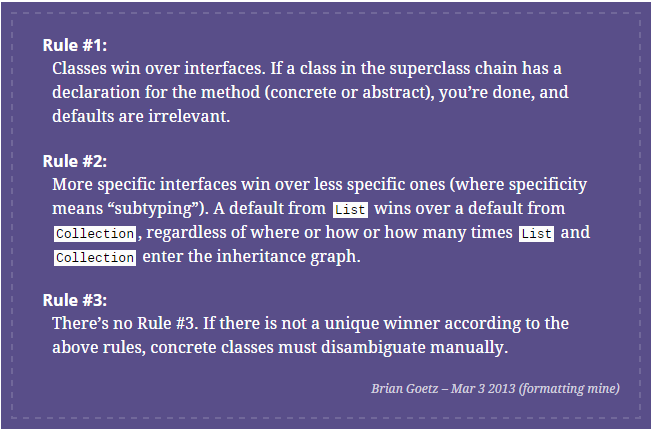
\includegraphics[width=5in]{screenshot.png}
\caption{Screenshot.}\label{screenshot_png}
\end{figure}

\haoyuan{I tried to understand the current algorithm, and did more experiments in eclipse.
Now I borrow some ideas from the current version, and give a new version of the algorithm in text. See below.

(1) I guess the function \textsf{tops} is not necessary. The first step is still
\[\textsf{mbody}(m,C_i)\in\overline{meth}\textrm{ (excluding \textbf{static} methods)}\]

(2) Assume the context is ``interface $C_0$ extends $\overline{C}$ \{$meth'$;...\}''. First handle
\[\textsf{override}(meth',\overline{meth}) \eqno{(*)}\]

(3) If $meth'\ne\none$, $(*)$ returns $meth'$ if
\[\forall meth\in\overline{meth},meth'\subtype meth\]
even if there are conflicts in $\overline{meth}$.

(4) If $meth'=\none$, we need to figure out
\[\textsf{mostSpecific}(\overline{meth})\]
and it should be the one that ``overrides'' all the others in $\overline{meth}$. It means we should not only deal with the return types of methods, but also look into the subtyping relation of interfaces. But for abstract methods, only return types are taken into consideration.
}
\end{comment}

%\text{\yanlin{shouldn't mostSpecific be: $\forall \method' \in \methods : \method \subtype
%  \method'$ ?}}

%(2) If $body_1.\textsf{returnType}=body_2.\textsf{returnType}$, \textsf{shadow} tends to return a default method. If both $body_1$ and $body_2$ are default methods, \textsf{shadow} throws an error.
%\begin{equation*}
%\begin{array}{ll}
%\textsf{shadow}(body_1, body_2)=\textsf{ERROR} & \textsf{if }body_1.\textsf{modifier}=body_2.\textsf{modifier}=\textbf{default}\\
%\textsf{shadow}(body_1, body_2)=body_1 \hspace{.1in} & \textsf{if }body_1.\textsf{modifier}=\textbf{default} \\
%\textsf{shadow}(body_1, body_2)=body_2 \hspace{.1in} & \textsf{if }body_2.\textsf{modifier}=\textbf{default} \\
%\textsf{shadow}(body_1, body_2)=body_1\textsf{ (or }body_2\textsf{)} \hspace{.1in} & \textsf{otherwise}
%\end{array}
%\end{equation*}
%
%(3) If $body_1.\textsf{returnType}<:body_2.\textsf{returnType}$, \textsf{shadow} tends to choose the one with the subtype (namely $body_1$), but only when both methods are abstract, otherwise it gives an error. The other direction $body_2.\textsf{returnType}<:body_1.\textsf{returnType}$ follows the same rule. It also gives an error if there is no subtyping relationship between two return types.
%\begin{equation*}
%\begin{array}{ll}
%\textsf{shadow}(body_1, body_2)=body_1 & \textsf{if }body_1.\textsf{modifier}=body_2.\textsf{modifier}=\emptyset\\
%& \textsf{and }body_1.\textsf{returnType}<:body_2.\textsf{returnType}\\
%\textsf{shadow}(body_1, body_2)=body_2 & \textsf{if }body_1.\textsf{modifier}=body_2.\textsf{modifier}=\emptyset\\
%& \textsf{and }body_2.\textsf{returnType}<:body_1.\textsf{returnType}\\
%\textsf{shadow}(body_1, body_2)=\textsf{ERROR} \hspace{.1in} & \textsf{otherwise}
%\end{array}
%\end{equation*}

%\subsubsection{Auxiliary function: \textsf{replace}}
%
%The \textsf{replace} function takes two same methods (with the same name and types of arguments), and gives the result of the first method overriding the second one.
%
%\begin{equation*}
%\begin{array}{ll}
%\textsf{replace}(body_1, body_2)=body_1 & \textsf{if }body_2=\emptyset\\
%\textsf{replace}(body_1, body_2)=body_2 & \textsf{if }body_1=\emptyset\\
%\textsf{replace}(body_1, body_2)=body_1 & \textsf{if }body_1.\textsf{returnType}<:body_2.\textsf{returnType}\\
%\textsf{replace}(body_1, body_2)=\textsf{ERROR} \hspace{.1in} & \textsf{otherwise}
%\end{array}
%\end{equation*}
